\documentclass{article}
\textheight 23.5cm \textwidth 15.8cm
%\leftskip -1cm
\topmargin -1.5cm \oddsidemargin 0.3cm \evensidemargin -0.3cm
%\documentclass[final]{siamltex}

\usepackage{ctex}
\usepackage{verbatim}
\usepackage{fancyhdr}
\usepackage{graphicx}
\usepackage{amsmath}
\usepackage{amssymb}
\usepackage{float}
\usepackage{multirow}
\usepackage{colortbl}
\usepackage{amsthm}
\usepackage{bm}
\usepackage{tikz}

\textheight 23.5cm \textwidth 15.8cm
\topmargin -1.5cm \oddsidemargin 0.3cm \evensidemargin -0.3cm
\title{HW5 实验报告}
\author{PB20010429 侯相龙}

\begin{document}
\maketitle
\section{实验内容}
实现如下文章中 Tutte 参数化:
Floater. Parametrization and smooth approximation of surface triangulations.
CAGD1997


\section{实验原理}
将网格映射到一个简单的几何形状(单位圆),并保持网格上相邻点之间的距离关系尽可能不变。

\section{算法介绍与步骤}
\begin{description}
    \item[1)]找到网格的边界,并将边界点的坐标固定在单位圆上的。
    \item[2)]构造拉普拉斯矩阵。对于每个网格顶点,计算其相邻顶点之间的连边数(1或0),并将其作为拉普拉斯矩阵的对应元素。最后,将对角线元素设置为相邻顶点的连边数的相反数。
    \item[3)]调整矩阵,使得边界点对应的对角元为1,对应行的非对角元为0 
    \item[4)]构造方程右端项,边界点对应{\bf1)}中构造的二维坐标,非边界点为0。
    \item[5)]将参数化坐标映射到目标几何形状。
\end{description}


\section{测试数据与实验结果}
对猫头网格(cathead.obj)进行测试,实验结果如下

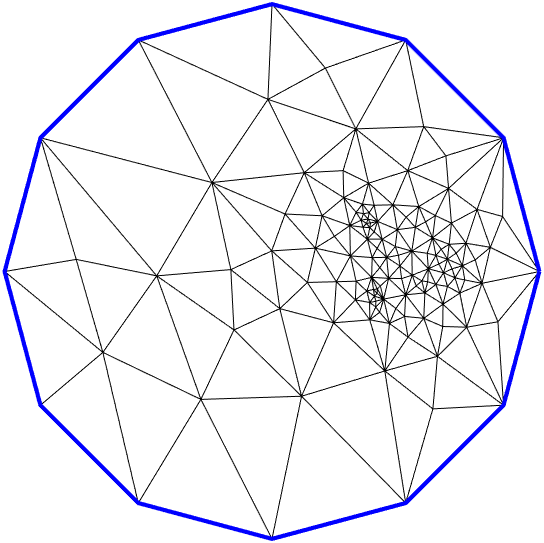
\includegraphics[width=0.7\linewidth]{1.png}



\end{document}
